\documentclass{standalone}
\usepackage{tikz}

\begin{document}
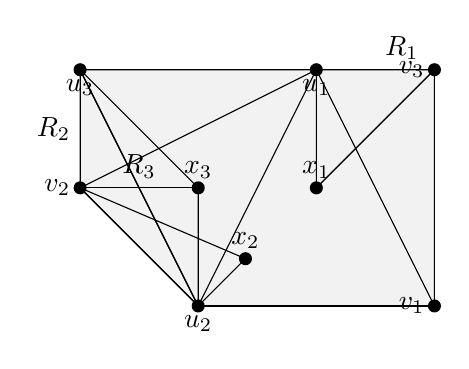
\begin{tikzpicture}[scale=1.5]
    % Points
    \def\uone{ (2,2) }
    \def\utwo{ (1,0) }
    \def\uthree{ (0,2) }
    \def\vone{ (3,0) }
    \def\vtwo{ (0,1) }
    \def\vthree{ (3,2) }
    \def\xone{ (2,1) }
    \def\xtwo{ (1.4,0.4) }
    \def\xthree{ (1,1) }

    % Regions
    \draw[fill=gray!10] (2,2) -- (3,0) -- (3,2) -- cycle node [pos=0.5, above right] {$R_1$};
    \draw[fill=gray!10] (0,2) -- (1,0) -- (0,1) -- cycle node [pos=0.5, left] {$R_2$};
    \draw[fill=gray!10] (0,2) -- (2,2) -- (3,2) -- (3,0) -- (1,0) -- cycle node [pos=0.5, above] {$R_3$};

    % Nodes
    \node[circle,fill=black,scale=0.5] at \uone {};
    \node[circle,fill=black,scale=0.5] at \utwo {};
    \node[circle,fill=black,scale=0.5] at \uthree {};
    \node[circle,fill=black,scale=0.5] at \vone {};
    \node[circle,fill=black,scale=0.5] at \vtwo {};
    \node[circle,fill=black,scale=0.5] at \vthree {};
    \node[circle,fill=black,scale=0.5] at \xone {};
    \node[circle,fill=black,scale=0.5] at \xtwo {};
    \node[circle,fill=black,scale=0.5] at \xthree {};

    % Labels
    \node[anchor=north] at \uone {$u_1$};
    \node[anchor=north] at \utwo {$u_2$};
    \node[anchor=north] at \uthree {$u_3$};
    \node[anchor=east] at \vone {$v_1$};
    \node[anchor=east] at \vtwo {$v_2$};
    \node[anchor=east] at \vthree {$v_3$};
    \node[anchor=south] at \xone {$x_1$};
    \node[anchor=south] at \xtwo {$x_2$};
    \node[anchor=south] at \xthree {$x_3$};

    % Edges
    \draw (2,2) -- (3,0);
    \draw (2,2) -- (1,0);
    \draw (2,2) -- (0,2);
    \draw (2,2) -- (3,2);
    \draw (3,2) -- (3,0);
    \draw (3,2) -- (0,2);
    \draw (0,2) -- (1,0);
    \draw (0,2) -- (0,1);
    \draw (0,1) -- (1,0);
    \draw (1,0) -- (3,0);
    \draw (0,1) -- (2,2); % Edge from (0,1) to (2,2) through x3, x2, etc.
    \draw (0,1) -- \xthree -- \utwo;
    \draw (0,1) -- \xtwo -- \utwo;
    \draw (0,1) -- \xthree;
    \draw (1,0) -- \xthree -- \utwo;
    \draw (1,0) -- \xthree -- \vtwo;
    \draw (1,0) -- \xthree -- \uthree;
    \draw (3,2) -- \xone -- \uone;
    \draw (3,2) -- \xone -- \vthree;
\end{tikzpicture}
\end{document}